\documentclass[a4paper, 10pt, twoside]{article}
\usepackage[left=2cm, right=2cm, top=2cm, bottom=3cm]{geometry}
\usepackage[super]{natbib}
\usepackage{amsmath}
\usepackage[shortlabels]{enumitem}
\usepackage{bbold}
\usepackage{graphicx}
\usepackage{url}
\usepackage{hyperref}
\hypersetup{
    colorlinks=true,
    linkcolor=blue,
    filecolor=magenta,      
    urlcolor=cyan,
}


\begin{document}

\title{High Performance Computing - Micro Aevol}
\author{T\'eo Bouvard}
\maketitle

\section{Introduction}

\section{Version CPU}

Dans cette partie, on étudie l'optimisation la version CPU du code d'Aevol. Le processeur utilisé est un AMD Ryzen 7 3700X avec 32GB de RAM DDR4 à 3200MHz, le code est compilé à l'aide de CMake 3.19.1, g++ 10.2.0 et OpenMP 4.5 (201511).

\subsection{Analyse}

Afin de se familiariser avec le code, il est intéressant de profiler son exécution. Cela permet d'identifier la structure globale du programme ainsi que son chemin critique.

\begin{figure}
	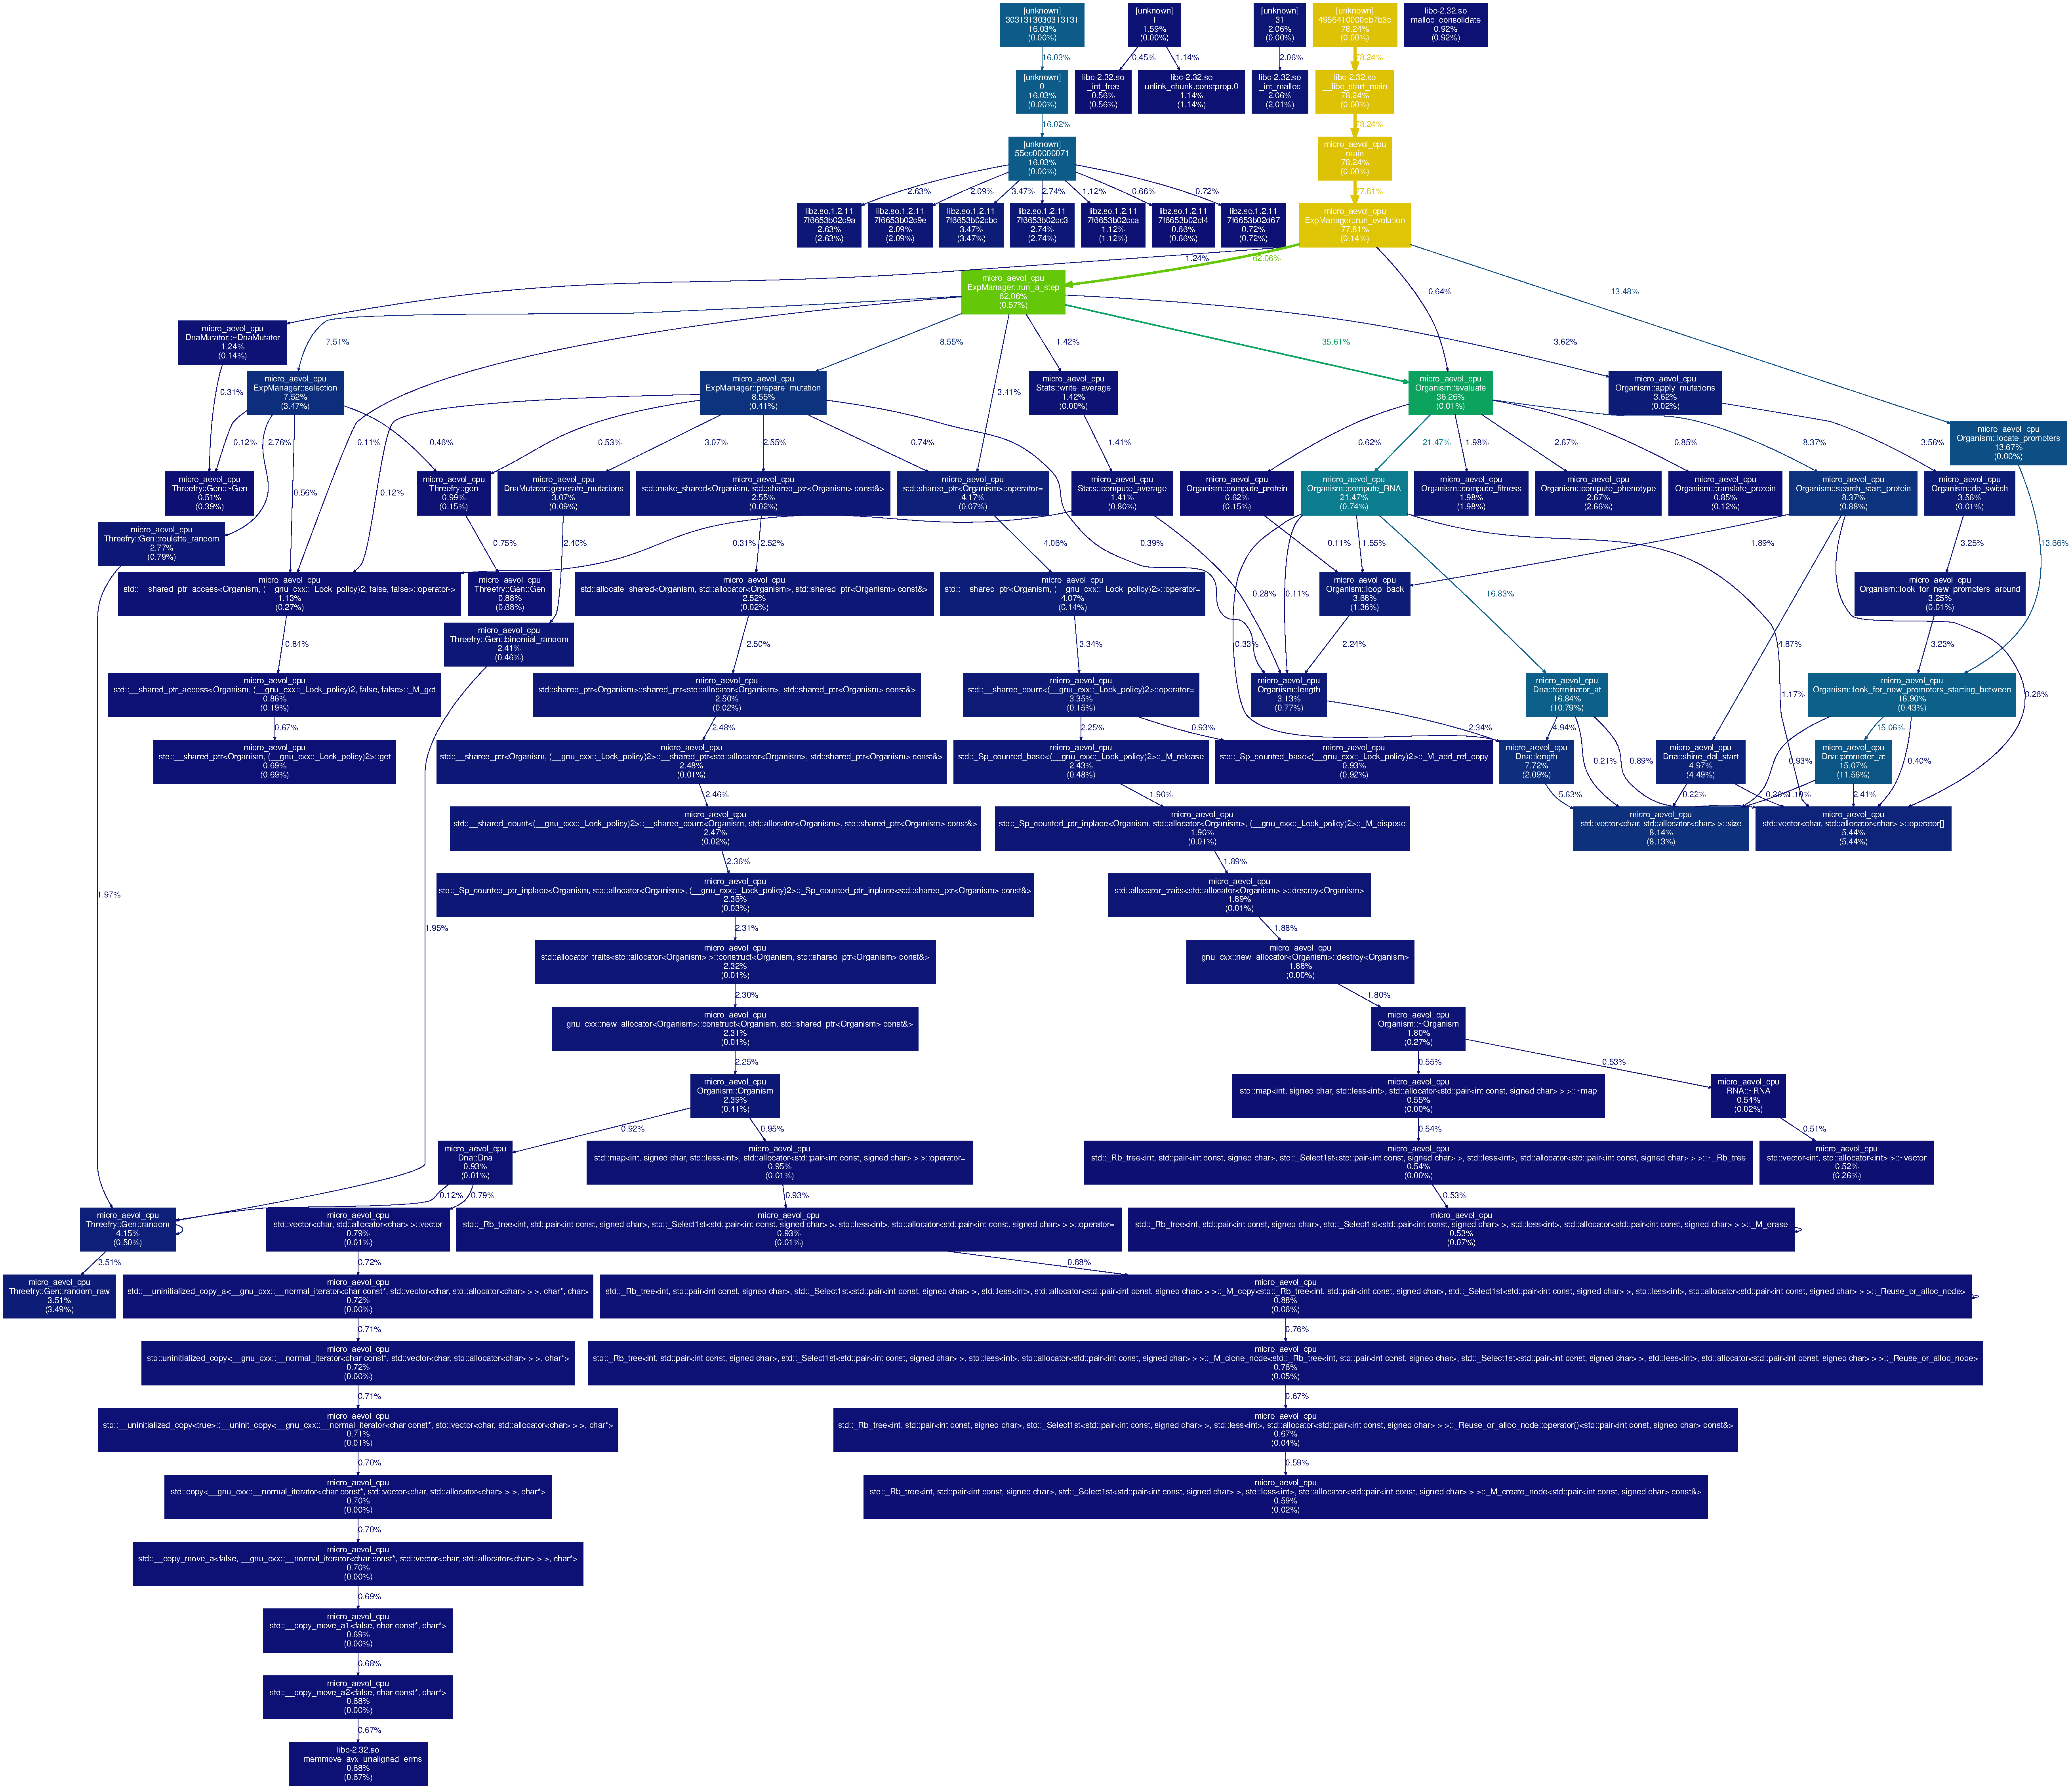
\includegraphics[width=\linewidth]{img/init_profile_debug.pdf}
	\caption{Profilage de l'application avec les paramètres par défaut à l'aide de \textit{perf}}
\end{figure}

Dans le cas d'Aevol, on remarque que la fonction \textit{run\_a\_step} est exécutée pour chaque pas de temps de \textit{run\_evolution}, dont le nombre d'itérations est spécifié par l'argument \textit{n\_steps}.
Dans cette fonction, les différentes étapes du modèle biologique sont exécutées pour chaque organisme.

\subsubsection*{Parallélisation du modèle}

Toutes les étapes de ce modèle sont indépendantes pour chaque organisme sauf l'étape de sélection qui requiert la lecture de l'état des organismes voisins sur la grille. Une optimisation naturelle est donc de paralléliser le traitement de chaque organisme\label{parallel/orga}.

\subsubsection*{Latence du disque}

Une autre simple optimisation est de limiter les appels à \textit{printf}, qui ralentissent l'exécution de manière significative lorsque ces derniers sont très fréquents. En effet, en utilisant les arguments par défaut on diminue de moitié le temps d'exécution en redirigeant la sortie standard ainsi que la sortie d'erreur vers \textit{/dev/null}. Bien évidemment, cette optimisation n'est pas aussi significative lorsque l'on utilise des tailles de problèmes plus élevées, mais il est sage d'éviter des appels systèmes coûteux lorsqu'ils ne sont pas nécessaires. Une alternative à la redirection des stream serait d'ajouter un argument permettant de contrôler la verbosité du programme, et ainsi s'affranchir du coût de tous ces appels systèmes lors d'une exécution en mode silencieux.

De manière similaire, les écritures dans les fichiers de statistiques invoquant \textit{std::endl} ou \textit{std::flush} imposent la synchronisation des flux de sortie, ce qui peut avoir un coût d'appel système assez élevé lié à la lenteur de l'écriture sur disque. Une meilleure solution serait de stocker les statistiques en mémoire jusqu'au point de backup afin de les écrire dans des fichiers en batch, ce qui améliorerait le buffering déja proposé par l'OS.

\subsection{Implémentation}

Dans l'optique de mesurer uniquement l'optimisation de la performance du modèle biologique, les benchmarks qui suivent n'incluent pas le temps d'écriture des fichiers de backup. En effet, cette écriture est réalisée par un seul thread et peut nécéssiter la compression DEFLATE de plusieurs GB de données à l'aide de zlib, ce qui influe de manière significative sur le temps d'exécution du programme. Cependant, c'est un coût qui n'est pas directement lié au modèle biologique que l'on cherche à optimiser, et qui n'est effectué qu'à chaque point de backup. Si l'on souhaitait optimiser cette partie du programme, il serait utile d'utiliser un algorithme de compression plus performant que DEFLATE tels que LZ4 ou zstd.

Chaque boucle itérant sur l'ensemble des organismes de la simulation est parallélisée à l'aide d'une directive \textit{omp parallel for}, en utilisant un scheduling statique. Ce choix de scheduling provient de l'observation de la répartition des charges de calcul sur les différents organismes.

\begin{itemize}
	\item Lors des phases de sélection, de swap de population et de recherche de meilleur individu, les calculs sont identiques pour chaque organisme.
	\item La phase d'évaluation n'est effectuée que si l'organisme a subi une mutation, ce qui est lié à un processus aléatoire. De plus, cette phase est d'autant plus couteuse que le nombre de mutations subies est élevé. Cependant, chaque organisme est soumis au même processus aléatoire de mutation, ce qui répartit les mutations de manière uniforme dans la population.
\end{itemize}

Ces deux observations suggèrent que la charge de calcul est répartie de manière uniforme sur l'ensemble de la population, et qu'il sera donc plus performant de diviser le traitement en chunks de taille égale plutot que d'opter pour des stratégies de scheduling dynamiques ou guidées qui nécéssiteraient un overhead inutile dans ce cas particulier.

\begin{figure}
	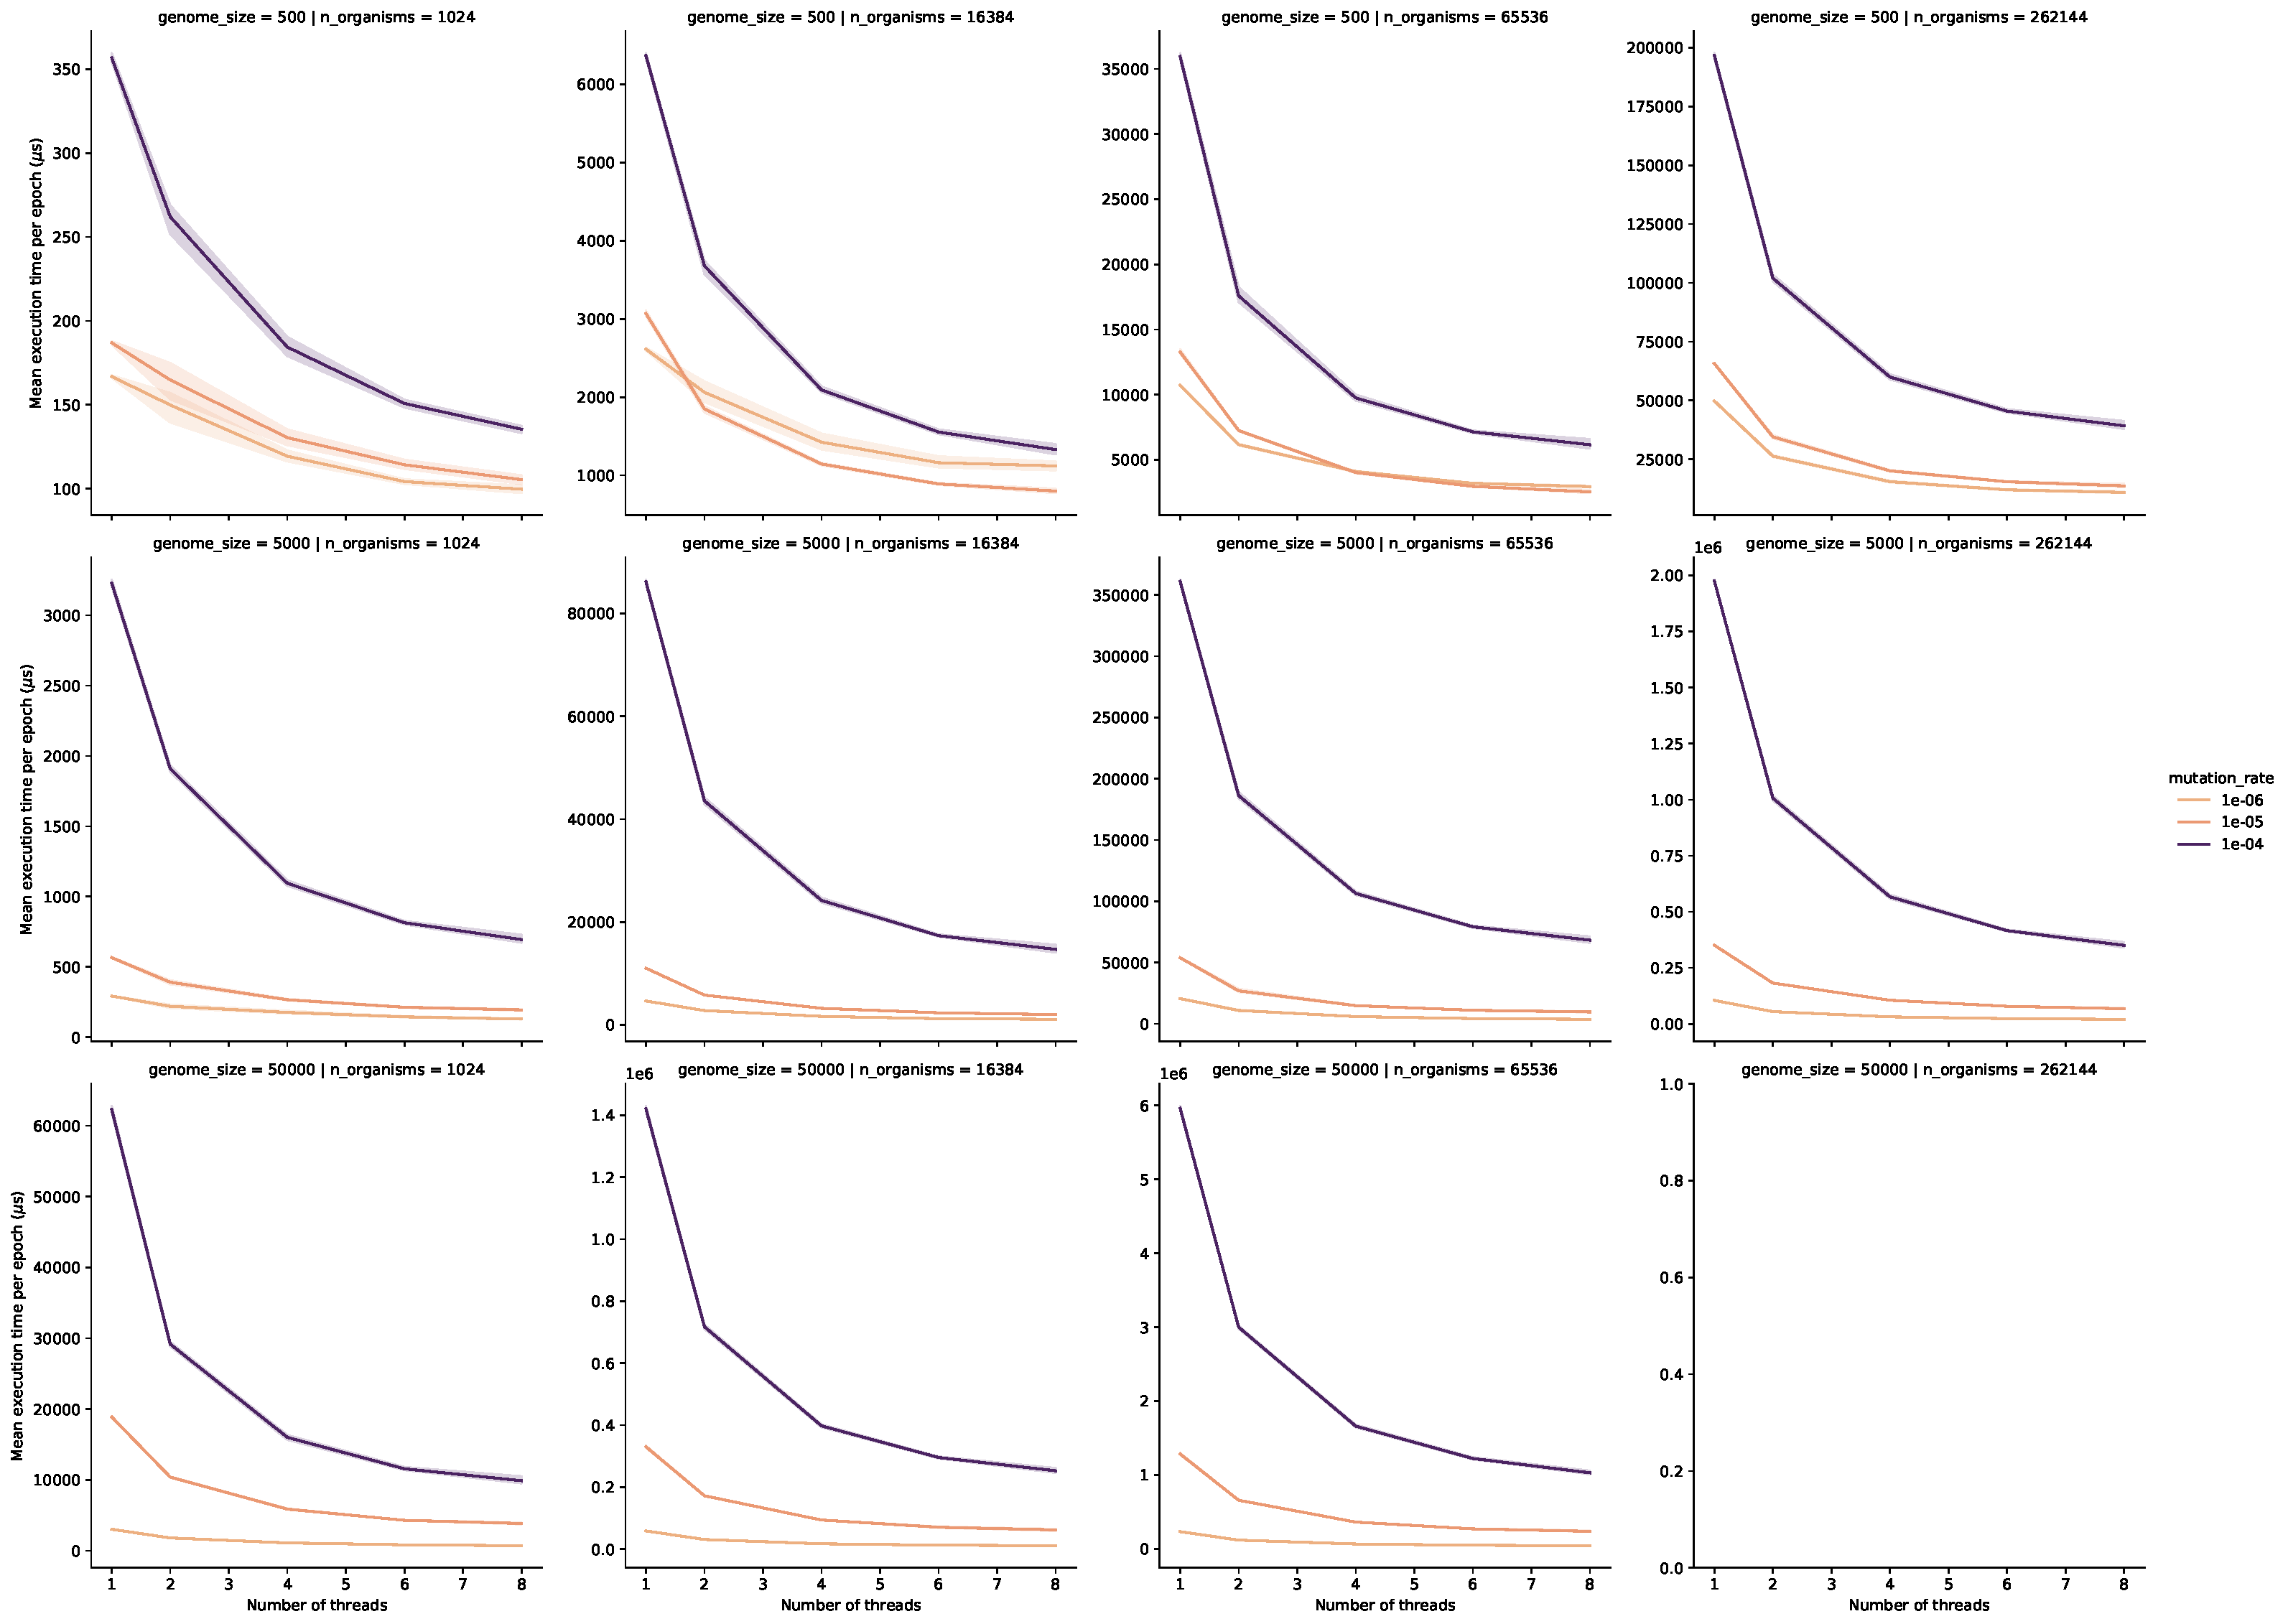
\includegraphics[width=\linewidth]{img/benchmark_omp_static.pdf}
	\caption{Benchmarks de la parallélisation du modèle biologique}
\end{figure}

La première observation qui peut être réalisée est que toutes choses étant égales par ailleurs, le temps d'éxécution du programme augmente avec le taux de mutation. Cela s'explique par la phase d'évaluation qui n'est effectuée qu'en cas de mutation. On observe aussi un passage à l'échelle fort de cette parallélisation, car le temps d'exécution est inversement proportionnel au nombre de threads utilisés.

\section{Version GPU}

Divergence \citep{nvidia/branching}



\bibliographystyle{unsrtnat}
\bibliography{report}

\end{document}
